% Options for packages loaded elsewhere
\PassOptionsToPackage{unicode}{hyperref}
\PassOptionsToPackage{hyphens}{url}
%
\documentclass[
  ngerman,
]{article}
\usepackage{amsmath,amssymb}
\usepackage{lmodern}
\usepackage{iftex}
\ifPDFTeX
  \usepackage[T1]{fontenc}
  \usepackage[utf8]{inputenc}
  \usepackage{textcomp} % provide euro and other symbols
\else % if luatex or xetex
  \usepackage{unicode-math}
  \defaultfontfeatures{Scale=MatchLowercase}
  \defaultfontfeatures[\rmfamily]{Ligatures=TeX,Scale=1}
\fi
% Use upquote if available, for straight quotes in verbatim environments
\IfFileExists{upquote.sty}{\usepackage{upquote}}{}
\IfFileExists{microtype.sty}{% use microtype if available
  \usepackage[]{microtype}
  \UseMicrotypeSet[protrusion]{basicmath} % disable protrusion for tt fonts
}{}
\makeatletter
\@ifundefined{KOMAClassName}{% if non-KOMA class
  \IfFileExists{parskip.sty}{%
    \usepackage{parskip}
  }{% else
    \setlength{\parindent}{0pt}
    \setlength{\parskip}{6pt plus 2pt minus 1pt}}
}{% if KOMA class
  \KOMAoptions{parskip=half}}
\makeatother
\usepackage{xcolor}
\IfFileExists{xurl.sty}{\usepackage{xurl}}{} % add URL line breaks if available
\IfFileExists{bookmark.sty}{\usepackage{bookmark}}{\usepackage{hyperref}}
\hypersetup{
  pdftitle={Spatial Analysis mit R (I)},
  pdflang={de},
  hidelinks,
  pdfcreator={LaTeX via pandoc}}
\urlstyle{same} % disable monospaced font for URLs
\usepackage{color}
\usepackage{fancyvrb}
\newcommand{\VerbBar}{|}
\newcommand{\VERB}{\Verb[commandchars=\\\{\}]}
\DefineVerbatimEnvironment{Highlighting}{Verbatim}{commandchars=\\\{\}}
% Add ',fontsize=\small' for more characters per line
\usepackage{framed}
\definecolor{shadecolor}{RGB}{248,248,248}
\newenvironment{Shaded}{\begin{snugshade}}{\end{snugshade}}
\newcommand{\AlertTok}[1]{\textcolor[rgb]{0.94,0.16,0.16}{#1}}
\newcommand{\AnnotationTok}[1]{\textcolor[rgb]{0.56,0.35,0.01}{\textbf{\textit{#1}}}}
\newcommand{\AttributeTok}[1]{\textcolor[rgb]{0.77,0.63,0.00}{#1}}
\newcommand{\BaseNTok}[1]{\textcolor[rgb]{0.00,0.00,0.81}{#1}}
\newcommand{\BuiltInTok}[1]{#1}
\newcommand{\CharTok}[1]{\textcolor[rgb]{0.31,0.60,0.02}{#1}}
\newcommand{\CommentTok}[1]{\textcolor[rgb]{0.56,0.35,0.01}{\textit{#1}}}
\newcommand{\CommentVarTok}[1]{\textcolor[rgb]{0.56,0.35,0.01}{\textbf{\textit{#1}}}}
\newcommand{\ConstantTok}[1]{\textcolor[rgb]{0.00,0.00,0.00}{#1}}
\newcommand{\ControlFlowTok}[1]{\textcolor[rgb]{0.13,0.29,0.53}{\textbf{#1}}}
\newcommand{\DataTypeTok}[1]{\textcolor[rgb]{0.13,0.29,0.53}{#1}}
\newcommand{\DecValTok}[1]{\textcolor[rgb]{0.00,0.00,0.81}{#1}}
\newcommand{\DocumentationTok}[1]{\textcolor[rgb]{0.56,0.35,0.01}{\textbf{\textit{#1}}}}
\newcommand{\ErrorTok}[1]{\textcolor[rgb]{0.64,0.00,0.00}{\textbf{#1}}}
\newcommand{\ExtensionTok}[1]{#1}
\newcommand{\FloatTok}[1]{\textcolor[rgb]{0.00,0.00,0.81}{#1}}
\newcommand{\FunctionTok}[1]{\textcolor[rgb]{0.00,0.00,0.00}{#1}}
\newcommand{\ImportTok}[1]{#1}
\newcommand{\InformationTok}[1]{\textcolor[rgb]{0.56,0.35,0.01}{\textbf{\textit{#1}}}}
\newcommand{\KeywordTok}[1]{\textcolor[rgb]{0.13,0.29,0.53}{\textbf{#1}}}
\newcommand{\NormalTok}[1]{#1}
\newcommand{\OperatorTok}[1]{\textcolor[rgb]{0.81,0.36,0.00}{\textbf{#1}}}
\newcommand{\OtherTok}[1]{\textcolor[rgb]{0.56,0.35,0.01}{#1}}
\newcommand{\PreprocessorTok}[1]{\textcolor[rgb]{0.56,0.35,0.01}{\textit{#1}}}
\newcommand{\RegionMarkerTok}[1]{#1}
\newcommand{\SpecialCharTok}[1]{\textcolor[rgb]{0.00,0.00,0.00}{#1}}
\newcommand{\SpecialStringTok}[1]{\textcolor[rgb]{0.31,0.60,0.02}{#1}}
\newcommand{\StringTok}[1]{\textcolor[rgb]{0.31,0.60,0.02}{#1}}
\newcommand{\VariableTok}[1]{\textcolor[rgb]{0.00,0.00,0.00}{#1}}
\newcommand{\VerbatimStringTok}[1]{\textcolor[rgb]{0.31,0.60,0.02}{#1}}
\newcommand{\WarningTok}[1]{\textcolor[rgb]{0.56,0.35,0.01}{\textbf{\textit{#1}}}}
\usepackage{longtable,booktabs,array}
\usepackage{calc} % for calculating minipage widths
% Correct order of tables after \paragraph or \subparagraph
\usepackage{etoolbox}
\makeatletter
\patchcmd\longtable{\par}{\if@noskipsec\mbox{}\fi\par}{}{}
\makeatother
% Allow footnotes in longtable head/foot
\IfFileExists{footnotehyper.sty}{\usepackage{footnotehyper}}{\usepackage{footnote}}
\makesavenoteenv{longtable}
\usepackage{graphicx}
\makeatletter
\def\maxwidth{\ifdim\Gin@nat@width>\linewidth\linewidth\else\Gin@nat@width\fi}
\def\maxheight{\ifdim\Gin@nat@height>\textheight\textheight\else\Gin@nat@height\fi}
\makeatother
% Scale images if necessary, so that they will not overflow the page
% margins by default, and it is still possible to overwrite the defaults
% using explicit options in \includegraphics[width, height, ...]{}
\setkeys{Gin}{width=\maxwidth,height=\maxheight,keepaspectratio}
% Set default figure placement to htbp
\makeatletter
\def\fps@figure{htbp}
\makeatother
\setlength{\emergencystretch}{3em} % prevent overfull lines
\providecommand{\tightlist}{%
  \setlength{\itemsep}{0pt}\setlength{\parskip}{0pt}}
\setcounter{secnumdepth}{5}
\ifXeTeX
  % Load polyglossia as late as possible: uses bidi with RTL langages (e.g. Hebrew, Arabic)
  \usepackage{polyglossia}
  \setmainlanguage[]{german}
\else
  \usepackage[main=ngerman]{babel}
% get rid of language-specific shorthands (see #6817):
\let\LanguageShortHands\languageshorthands
\def\languageshorthands#1{}
\fi
\ifLuaTeX
  \usepackage{selnolig}  % disable illegal ligatures
\fi

\title{Spatial Analysis mit R (I)}
\usepackage{etoolbox}
\makeatletter
\providecommand{\subtitle}[1]{% add subtitle to \maketitle
  \apptocmd{\@title}{\par {\large #1 \par}}{}{}
}
\makeatother
\subtitle{Methodenwoche}
\author{true}
\date{20.--21. September 2021}

\begin{document}
\maketitle

{
\setcounter{tocdepth}{2}
\tableofcontents
}
\hypertarget{zeitplan}{%
\section*{Zeitplan}\label{zeitplan}}
\addcontentsline{toc}{section}{Zeitplan}

Alle Sitzungen finden über Zoom statt.

\begin{longtable}[]{@{}
  >{\raggedright\arraybackslash}p{(\columnwidth - 4\tabcolsep) * \real{0.1667}}
  >{\raggedright\arraybackslash}p{(\columnwidth - 4\tabcolsep) * \real{0.4167}}
  >{\raggedright\arraybackslash}p{(\columnwidth - 4\tabcolsep) * \real{0.4167}}@{}}
\toprule
\begin{minipage}[b]{\linewidth}\raggedright
Zeit
\end{minipage} & \begin{minipage}[b]{\linewidth}\raggedright
Montag
\end{minipage} & \begin{minipage}[b]{\linewidth}\raggedright
Dienstag
\end{minipage} \\
\midrule
\endhead
10:00--11:30 & \textbf{(1) \protect\hyperlink{getting-started}{Getting started} (LAS)} & \textbf{(5) Geodaten verschneiden: FTR} \\
\emph{11:30--11:45} & \emph{Kaffeepause} & \emph{Kaffeepause} \\
11:45--13:15 & \textbf{(2) \protect\hyperlink{daten-visualisieren}{Daten visualisieren} (FTR, HOS)} & \textbf{(6) Geodaten verschneiden: HOS, SYW} \\
\emph{13:15--14:15} & \emph{Mittagspause} & \emph{Mittagspause} \\
14:15--15:45 & \textbf{(3) \protect\hyperlink{karten-erstellen-ftr}{Karten erstellen} (FTR)} & \textbf{(7) Nach Hilfe fragen und und publizieren (FTR)} \\
\emph{15:45--16:15} & \emph{Kaffeepause} & \emph{Kaffeepause} \\
16:15--18:00 & \textbf{(4) \protect\hyperlink{karten-erstellen-hos}{Karten erstellen} (HOS, SYW)} & \textbf{(8) Looking back, looking ahead (LAS)} \\
\bottomrule
\end{longtable}

\hypertarget{getting-started}{%
\section{Getting started}\label{getting-started}}

\hypertarget{formales}{%
\subsection{Formales}\label{formales}}

\hypertarget{keine-reguluxe4re-anrechnung-des-workshops}{%
\subsubsection{Keine reguläre Anrechnung des Workshops}\label{keine-reguluxe4re-anrechnung-des-workshops}}

\begin{itemize}
\tightlist
\item
  Die Methodenwoche ist eine außercurriculare Veranstaltung
\item
  Keine Anrechnung als Prüfungsleistung für das reguläre Studium
\item
  Alle Teilnehmer*innen erhalten Methodenzentrum eine Bescheinigung über die erbrachte Leistung (Ende 2021/Anfang 2022)
\end{itemize}

\hypertarget{methodenzertifikat}{%
\subsubsection{Methodenzertifikat}\label{methodenzertifikat}}

\begin{itemize}
\tightlist
\item
  Nur für Bachelor-Studierende der Fachbereiche 02--05
\item
  Kann mit 5 CP beantragt werden
\item
  z.~B. Teilnahme Workshop (2 CP) + Leistungsnachweis (3 CP)
\item
  Maximal 20\% Fehlzeit zulässig für Teilnahmenachweis
\item
  Schriftliche Leistungsnachweise mit maximal vierwöchiger Abgabefrist
\item
  Alle Fragen dazu bitte an \href{mailto:hiwis-methodenzentrum@uni-frankfurt.de}{\nolinkurl{hiwis-methodenzentrum@uni-frankfurt.de}}
\end{itemize}

\hypertarget{inhaltliches}{%
\subsection{Inhaltliches}\label{inhaltliches}}

\hypertarget{lernziele-der-veranstaltung}{%
\subsubsection{Lernziele der Veranstaltung}\label{lernziele-der-veranstaltung}}

Sie können\ldots{}

\begin{itemize}
\tightlist
\item
  Datenvisualisierungen nachvollziehen und selbst gestalten.
\item
  Geodaten einlesen, transformieren und verschneiden.
\item
  Geodaten kartographisch darstellen.
\item
  Reproducible examples erstellen um nach Hilfe zu fragen.
\item
  Berichte in Rmarkdown verfassen und rendern.
\end{itemize}

\hypertarget{seminarkonzept}{%
\subsection{Seminarkonzept}\label{seminarkonzept}}

\begin{itemize}
\tightlist
\item
  Kompetenter Umgang mit Geodaten als Kernziel
\item
  Aber nicht im luftleeren Raum
\item
  Das Drumherum ist mindestens genauso wichtig
\item
  Unterlagen sind Auszüge aus einem zweisemestrigen Seminar
\end{itemize}

\hypertarget{opinionated}{%
\subsection{\texorpdfstring{``Opinionated\ldots{}''}{``Opinionated\ldots''}}\label{opinionated}}

\begin{itemize}
\tightlist
\item
  package choices:

  \begin{itemize}
  \tightlist
  \item
    \texttt{tidyverse}
  \item
    \texttt{sf}
  \end{itemize}
\item
  coding style:

  \begin{itemize}
  \tightlist
  \item
    Functional
  \item
    Pipes \texttt{\%\textgreater{}\%}
  \end{itemize}
\item
  workflow:

  \begin{itemize}
  \tightlist
  \item
    Incremental commands
  \item
    Rmarkdown (reproducible research)
  \end{itemize}
\end{itemize}

\hypertarget{didaktisches}{%
\subsection{Didaktisches}\label{didaktisches}}

\hypertarget{herausforderungen-in-der-it-didaktik}{%
\subsubsection{Herausforderungen in der IT-Didaktik}\label{herausforderungen-in-der-it-didaktik}}

\begin{itemize}
\tightlist
\item
  Unterschiedliche Erfahrungen, Kompetenzen und Herangehensweisen
\item
  Die eine Hälfte versteht gar nichts, die andere langweilt sich
\item
  Kleinster gemeinsamer Nenner: Schritt-für-Schritt-Anleitungen
\item
  In der Praxis wertlos
\end{itemize}

\hypertarget{everyone-fails}{%
\subsubsection{Everyone fails}\label{everyone-fails}}

\begin{itemize}
\tightlist
\item
  In der Praxis stoßen alle ständig an die Grenzen ihrer technischen Kompetenz.
\item
  Es geht darum, sich am Limit einigermaßen wohl zu fühlen und die Grenzen zu verschieben.
\item
  Gute Angewohnheiten (Strukturen, Formate, Stil) helfen dabei!
\end{itemize}

\hypertarget{mein-ansatz-in-der-lehre}{%
\subsubsection{Mein Ansatz in der Lehre}\label{mein-ansatz-in-der-lehre}}

\begin{itemize}
\tightlist
\item
  Strategische Überforderung durch schwierige Aufgaben?
\item
  Lösungsorientierte Didaktik!
\item
  Die affektive Seite (Spaß, Frust) ernst nehmen und thematisieren
\item
  Frustrationsschwelle trainieren
\end{itemize}

\hypertarget{schattenkompetenzen}{%
\subsubsection{``Schattenkompetenzen''}\label{schattenkompetenzen}}

\begin{itemize}
\tightlist
\item
  Fehlermeldungen lesen
\item
  Gezielt googlen (und Antworten auswählen)
\item
  Copy, paste, customize
\item
  Gute Fragen (online) stellen
\end{itemize}

\hypertarget{dieser-workshop-findet-in-verschiedenen-modi-statt}{%
\subsubsection{Dieser Workshop findet in verschiedenen Modi statt:}\label{dieser-workshop-findet-in-verschiedenen-modi-statt}}

\hypertarget{listen-and-share-las}{%
\paragraph{Listen and share (LAS)}\label{listen-and-share-las}}

\begin{itemize}
\tightlist
\item
  Ich rede (mit Folien oder ohne) oder moderiere eine Diskussion.
\item
  Sie hören mir und Ihren Kommiliton*innen aufmerksam zu.
\item
  Sie ``melden'' sich für Redebeiträge oder Fragen (Zoom-Funktion).
\end{itemize}

\hypertarget{follow-the-recipe-ftr}{%
\paragraph{Follow the recipe (FTR)}\label{follow-the-recipe-ftr}}

\begin{itemize}
\tightlist
\item
  Ich teile ein unvollständiges Beispielprojekt.
\item
  Wir gehen die Teilschritte nach und nach durch.
\item
  Ich ``habe den Plan'', stelle aber immer wieder Fragen ans Plenum.
\item
  Sie vollziehen die Schritte an Ihrer eigenen Kopie des Projekts nach.
\item
  Sie unterbrechen mich mit Nachfragen oder Problemen.
\end{itemize}

\hypertarget{hands-on-session-hos}{%
\paragraph{Hands-on session (HOS)}\label{hands-on-session-hos}}

\begin{itemize}
\tightlist
\item
  Sie bearbeiten praktische Aufgabenstellungen alleine.
\item
  Dabei sind sie in zufälligen Dreier-Konstellationen (Breakout-Session).
\item
  Bei Fragen oder Problemen wenden Sie sich zunächst an Ihre Kleingruppe.
\item
  Falls Sie nicht weiterkommen, fordern Sie Hilfe an (Zoom-Funktion).
\item
  Ich reagiere auf Hilfegesuche oder ``mache die Runde''.
\end{itemize}

\hypertarget{share-your-work-syw}{%
\paragraph{Share your work (SYW)}\label{share-your-work-syw}}

\begin{itemize}
\tightlist
\item
  Ich wähle eine Teilnehmer*in zufällig aus.
\item
  Die Person teilt ihren Bildschirm und berichtet von ihrer Bearbeitung eines Problems.
\item
  Alle anderen unterstützen solidarisch durch aktives Nachvollziehen, Nachfragen und Hinweise.
\end{itemize}

\hypertarget{technisches}{%
\subsection{Technisches}\label{technisches}}

\hypertarget{arbeitsplatz}{%
\subsubsection{Arbeitsplatz}\label{arbeitsplatz}}

\begin{itemize}
\tightlist
\item
  Challenge: Zoom (meinen Bildschirm) und R gleichzeitig sehen
\item
  Am allerbesten: Zweiter Bildschirm
\item
  Auch gut: Zweites Gerät (Tablet)
\end{itemize}

\hypertarget{workshopunterlagen}{%
\subsubsection{Workshopunterlagen}\label{workshopunterlagen}}

\begin{itemize}
\tightlist
\item
  Bookdown (statt OLAT)
\item
  \textsubscript{Können} Werden sich verändern
\item
  Am besten neu laden mit Strg+Umschalt+R
\item
  \url{https://tiny.gu/mwsa}
\end{itemize}

\hypertarget{rstudio-cloud}{%
\subsubsection{RStudio Cloud}\label{rstudio-cloud}}

\begin{itemize}
\tightlist
\item
  Grundsätzliche Empfehlung: R und RStudio lokal installieren
\item
  Wir nutzen im Rahmen des Workshops die RStudio Cloud

  \begin{itemize}
  \tightlist
  \item
    für einfaches Teilen von Code
  \item
    für homogenes Setup
  \end{itemize}
\end{itemize}

\hypertarget{daten-visualisieren}{%
\section{Daten visualisieren}\label{daten-visualisieren}}

\hypertarget{lernziele-dieser-sitzung}{%
\subsection{Lernziele dieser Sitzung}\label{lernziele-dieser-sitzung}}

Sie können\ldots{}

\begin{itemize}
\tightlist
\item
  einfache Befehle zur Visualisierung in Base R anwenden.
\item
  die Grammatik von \texttt{ggplot2} für Visualisierungen in Grundzügen wiedergeben und anwenden.
\item
  eigene Ideen für Visualisierungen entwickeln und umsetzen.
\end{itemize}

\hypertarget{voraussetzungen}{%
\subsection{Voraussetzungen}\label{voraussetzungen}}

Für diese Lektion benötigen wir das Paket \texttt{tidyverse}:

\begin{Shaded}
\begin{Highlighting}[]
\FunctionTok{library}\NormalTok{(tidyverse)}
\end{Highlighting}
\end{Shaded}

Und einen Datensatz, der in Form eines tibble vorliegt. Der Beispieldatensatz \texttt{diamonds} wird mitgeliefert:

\begin{Shaded}
\begin{Highlighting}[]
\NormalTok{diamonds}
\DocumentationTok{\#\# \# A tibble: 53,940 x 10}
\DocumentationTok{\#\#    carat cut       color clarity depth table price     x     y     z}
\DocumentationTok{\#\#    \textless{}dbl\textgreater{} \textless{}ord\textgreater{}     \textless{}ord\textgreater{} \textless{}ord\textgreater{}   \textless{}dbl\textgreater{} \textless{}dbl\textgreater{} \textless{}int\textgreater{} \textless{}dbl\textgreater{} \textless{}dbl\textgreater{} \textless{}dbl\textgreater{}}
\DocumentationTok{\#\#  1  0.23 Ideal     E     SI2      61.5    55   326  3.95  3.98  2.43}
\DocumentationTok{\#\#  2  0.21 Premium   E     SI1      59.8    61   326  3.89  3.84  2.31}
\DocumentationTok{\#\#  3  0.23 Good      E     VS1      56.9    65   327  4.05  4.07  2.31}
\DocumentationTok{\#\#  4  0.29 Premium   I     VS2      62.4    58   334  4.2   4.23  2.63}
\DocumentationTok{\#\#  5  0.31 Good      J     SI2      63.3    58   335  4.34  4.35  2.75}
\DocumentationTok{\#\#  6  0.24 Very Good J     VVS2     62.8    57   336  3.94  3.96  2.48}
\DocumentationTok{\#\#  7  0.24 Very Good I     VVS1     62.3    57   336  3.95  3.98  2.47}
\DocumentationTok{\#\#  8  0.26 Very Good H     SI1      61.9    55   337  4.07  4.11  2.53}
\DocumentationTok{\#\#  9  0.22 Fair      E     VS2      65.1    61   337  3.87  3.78  2.49}
\DocumentationTok{\#\# 10  0.23 Very Good H     VS1      59.4    61   338  4     4.05  2.39}
\DocumentationTok{\#\# \# ... with 53,930 more rows}
\end{Highlighting}
\end{Shaded}

Wenn wir mögen, können wir ihn mit der Funktion \texttt{data()} explizit in unser Environment laden:

\begin{Shaded}
\begin{Highlighting}[]
\FunctionTok{data}\NormalTok{(diamonds)}
\end{Highlighting}
\end{Shaded}

\hypertarget{uxfcberblick}{%
\subsection{Überblick}\label{uxfcberblick}}

Einen ersten Überblick kriegen wir zum Einen durch den Befehl \texttt{str()}, der uns die Typen in den Spalten anzeigt:

\begin{Shaded}
\begin{Highlighting}[]
\FunctionTok{str}\NormalTok{(diamonds)}
\DocumentationTok{\#\# tibble [53,940 x 10] (S3: tbl\_df/tbl/data.frame)}
\DocumentationTok{\#\#  $ carat  : num [1:53940] 0.23 0.21 0.23 0.29 0.31 0.24 0.24 0.26 0.22 0.23 ...}
\DocumentationTok{\#\#  $ cut    : Ord.factor w/ 5 levels "Fair"\textless{}"Good"\textless{}..: 5 4 2 4 2 3 3 3 1 3 ...}
\DocumentationTok{\#\#  $ color  : Ord.factor w/ 7 levels "D"\textless{}"E"\textless{}"F"\textless{}"G"\textless{}..: 2 2 2 6 7 7 6 5 2 5 ...}
\DocumentationTok{\#\#  $ clarity: Ord.factor w/ 8 levels "I1"\textless{}"SI2"\textless{}"SI1"\textless{}..: 2 3 5 4 2 6 7 3 4 5 ...}
\DocumentationTok{\#\#  $ depth  : num [1:53940] 61.5 59.8 56.9 62.4 63.3 62.8 62.3 61.9 65.1 59.4 ...}
\DocumentationTok{\#\#  $ table  : num [1:53940] 55 61 65 58 58 57 57 55 61 61 ...}
\DocumentationTok{\#\#  $ price  : int [1:53940] 326 326 327 334 335 336 336 337 337 338 ...}
\DocumentationTok{\#\#  $ x      : num [1:53940] 3.95 3.89 4.05 4.2 4.34 3.94 3.95 4.07 3.87 4 ...}
\DocumentationTok{\#\#  $ y      : num [1:53940] 3.98 3.84 4.07 4.23 4.35 3.96 3.98 4.11 3.78 4.05 ...}
\DocumentationTok{\#\#  $ z      : num [1:53940] 2.43 2.31 2.31 2.63 2.75 2.48 2.47 2.53 2.49 2.39 ...}
\end{Highlighting}
\end{Shaded}

Zum Anderen gibt die Hilfefunktion Auskunft über den Datensatz und die einzelnen Variablen (Metadaten):

\begin{Shaded}
\begin{Highlighting}[]
\NormalTok{?diamonds}
\end{Highlighting}
\end{Shaded}

Einen Überblick über die wichtigsten statistischen Parameter erhalten wir mit:

\begin{Shaded}
\begin{Highlighting}[]
\FunctionTok{summary}\NormalTok{(diamonds)}
\DocumentationTok{\#\#      carat               cut        color        clarity          depth      }
\DocumentationTok{\#\#  Min.   :0.2000   Fair     : 1610   D: 6775   SI1    :13065   Min.   :43.00  }
\DocumentationTok{\#\#  1st Qu.:0.4000   Good     : 4906   E: 9797   VS2    :12258   1st Qu.:61.00  }
\DocumentationTok{\#\#  Median :0.7000   Very Good:12082   F: 9542   SI2    : 9194   Median :61.80  }
\DocumentationTok{\#\#  Mean   :0.7979   Premium  :13791   G:11292   VS1    : 8171   Mean   :61.75  }
\DocumentationTok{\#\#  3rd Qu.:1.0400   Ideal    :21551   H: 8304   VVS2   : 5066   3rd Qu.:62.50  }
\DocumentationTok{\#\#  Max.   :5.0100                     I: 5422   VVS1   : 3655   Max.   :79.00  }
\DocumentationTok{\#\#                                     J: 2808   (Other): 2531                  }
\DocumentationTok{\#\#      table           price             x                y         }
\DocumentationTok{\#\#  Min.   :43.00   Min.   :  326   Min.   : 0.000   Min.   : 0.000  }
\DocumentationTok{\#\#  1st Qu.:56.00   1st Qu.:  950   1st Qu.: 4.710   1st Qu.: 4.720  }
\DocumentationTok{\#\#  Median :57.00   Median : 2401   Median : 5.700   Median : 5.710  }
\DocumentationTok{\#\#  Mean   :57.46   Mean   : 3933   Mean   : 5.731   Mean   : 5.735  }
\DocumentationTok{\#\#  3rd Qu.:59.00   3rd Qu.: 5324   3rd Qu.: 6.540   3rd Qu.: 6.540  }
\DocumentationTok{\#\#  Max.   :95.00   Max.   :18823   Max.   :10.740   Max.   :58.900  }
\DocumentationTok{\#\#                                                                   }
\DocumentationTok{\#\#        z         }
\DocumentationTok{\#\#  Min.   : 0.000  }
\DocumentationTok{\#\#  1st Qu.: 2.910  }
\DocumentationTok{\#\#  Median : 3.530  }
\DocumentationTok{\#\#  Mean   : 3.539  }
\DocumentationTok{\#\#  3rd Qu.: 4.040  }
\DocumentationTok{\#\#  Max.   :31.800  }
\DocumentationTok{\#\# }
\end{Highlighting}
\end{Shaded}

\hypertarget{visualisierung-mit-dem-standardpaket}{%
\subsection{Visualisierung mit dem Standardpaket}\label{visualisierung-mit-dem-standardpaket}}

Es gibt in R mehrere grundlegend verschiedene Möglichkeiten, Daten zu visualisieren. Für einen schnellen Überblick sind z.B. \texttt{hist()} und \texttt{boxplot()} hilfreich:

\begin{Shaded}
\begin{Highlighting}[]
\FunctionTok{hist}\NormalTok{(diamonds}\SpecialCharTok{$}\NormalTok{price)}
\end{Highlighting}
\end{Shaded}

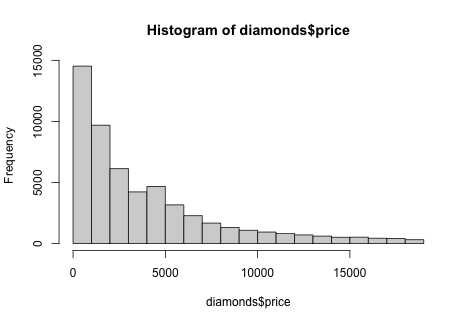
\includegraphics{_main_files/figure-latex/unnamed-chunk-8-1.png}

\begin{Shaded}
\begin{Highlighting}[]
\FunctionTok{boxplot}\NormalTok{(diamonds}\SpecialCharTok{$}\NormalTok{x)}
\end{Highlighting}
\end{Shaded}

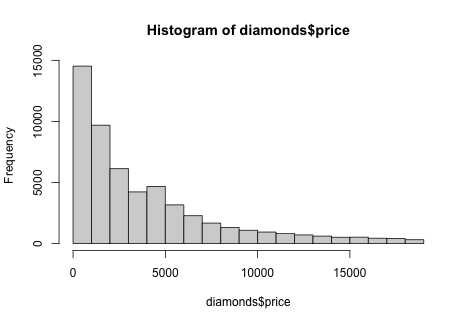
\includegraphics{_main_files/figure-latex/unnamed-chunk-9-1.png}

\hypertarget{visualisierung-mit-ggplot}{%
\subsection{\texorpdfstring{Visualisierung mit \texttt{ggplot()}}{Visualisierung mit ggplot()}}\label{visualisierung-mit-ggplot}}

Das Paket \texttt{ggplot2} ist Teil vom \texttt{tidyverse}. Hiermit lassen sich sehr flexible Graphiken gestalten. Wir werden ausschließlich mit diesem System arbeiten.

Die Syntax ist dabei auf den ersten Blick etwas komplexer.

Am Anfang steht der Befehl \texttt{ggplot(x)} mit dem Datensatz als Parameter

\begin{Shaded}
\begin{Highlighting}[]
\FunctionTok{ggplot}\NormalTok{(}\AttributeTok{data =}\NormalTok{ diamonds)}
\end{Highlighting}
\end{Shaded}


\includegraphics{_main_files/figure-latex/unnamed-chunk-10-1.png}

Mit einem Mapping-Parameter legen wir die Dimensionen fest:

\begin{Shaded}
\begin{Highlighting}[]
\FunctionTok{ggplot}\NormalTok{(}\AttributeTok{data =}\NormalTok{ diamonds, }\AttributeTok{mapping =} \FunctionTok{aes}\NormalTok{(}\AttributeTok{x =}\NormalTok{ price, }\AttributeTok{y =}\NormalTok{ carat))}
\end{Highlighting}
\end{Shaded}

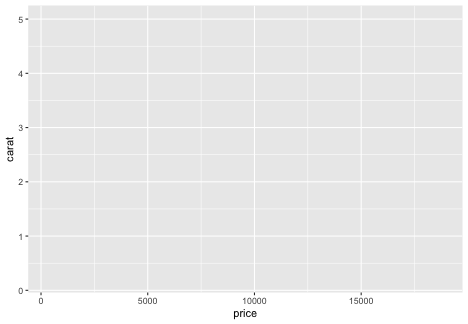
\includegraphics{_main_files/figure-latex/unnamed-chunk-11-1.png}

Das gleiche ohne Parameternamen:

\begin{Shaded}
\begin{Highlighting}[]
\FunctionTok{ggplot}\NormalTok{(diamonds, }\FunctionTok{aes}\NormalTok{(price, carat))}
\end{Highlighting}
\end{Shaded}

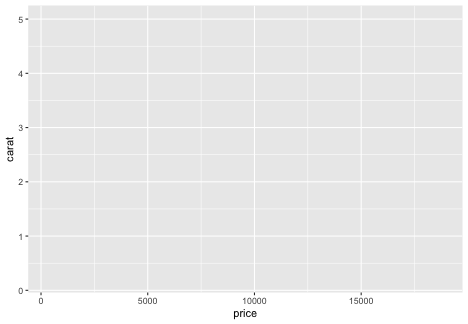
\includegraphics{_main_files/figure-latex/unnamed-chunk-12-1.png}

Nun kann mit dem \texttt{+}-Operator ein ``geometrischer'' Layer hinzugefügt werden:

\begin{Shaded}
\begin{Highlighting}[]
\FunctionTok{ggplot}\NormalTok{(diamonds, }\FunctionTok{aes}\NormalTok{(}\AttributeTok{x =}\NormalTok{ carat, }\AttributeTok{y =}\NormalTok{ price)) }\SpecialCharTok{+}
  \FunctionTok{geom\_point}\NormalTok{()}
\end{Highlighting}
\end{Shaded}

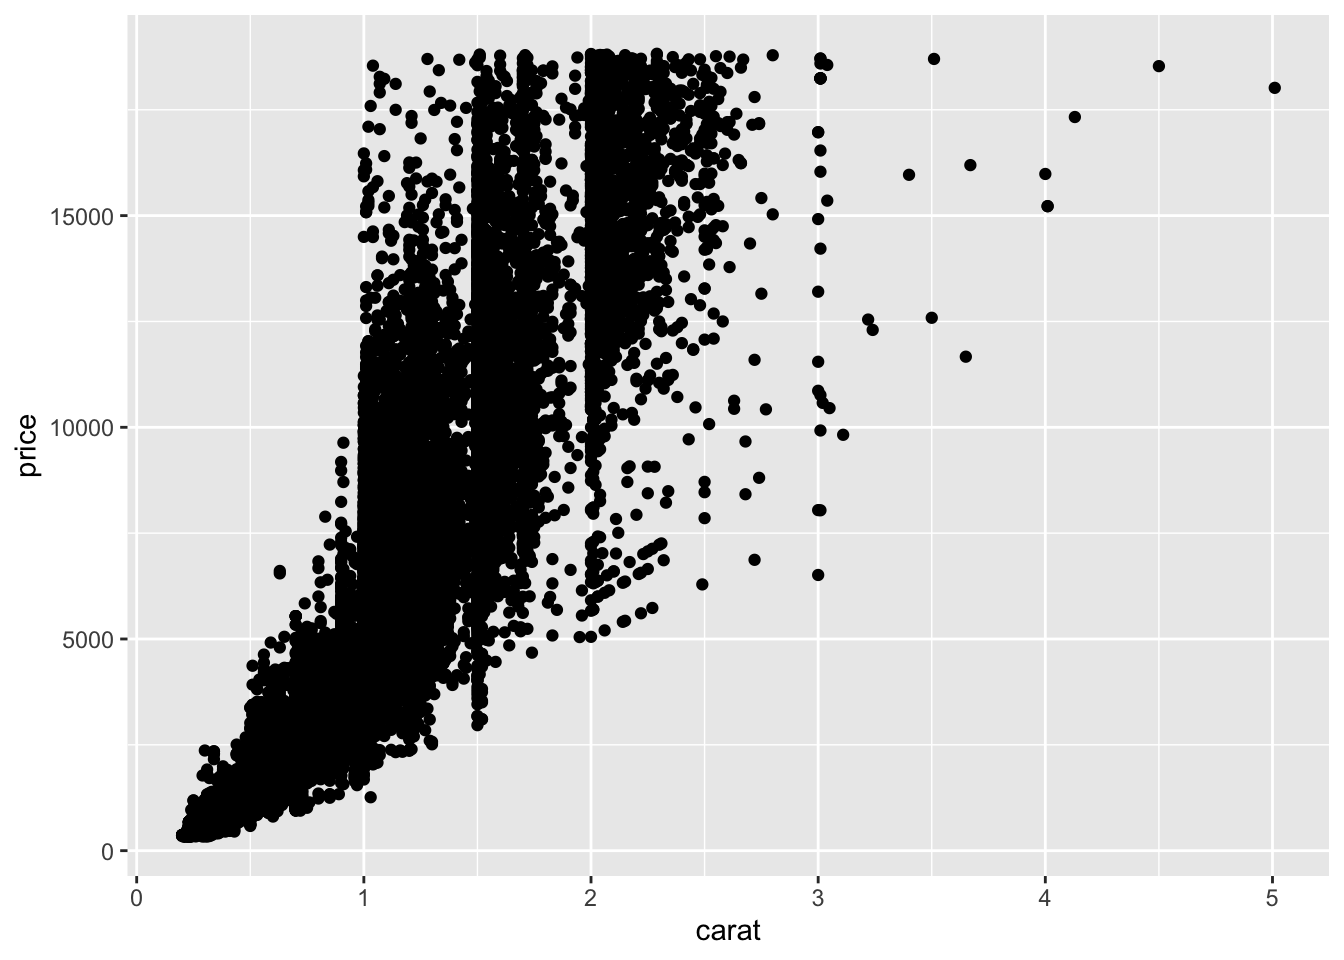
\includegraphics{_main_files/figure-latex/unnamed-chunk-13-1.png}

Weitere \texttt{geom}-Layer lassen sich mit dem \texttt{+}-Operator hinzufügen:

\begin{Shaded}
\begin{Highlighting}[]
\FunctionTok{ggplot}\NormalTok{(diamonds, }\FunctionTok{aes}\NormalTok{(}\AttributeTok{x =}\NormalTok{ carat, }\AttributeTok{y =}\NormalTok{ price)) }\SpecialCharTok{+}
  \FunctionTok{geom\_point}\NormalTok{() }\SpecialCharTok{+}
  \FunctionTok{geom\_smooth}\NormalTok{()}
\end{Highlighting}
\end{Shaded}

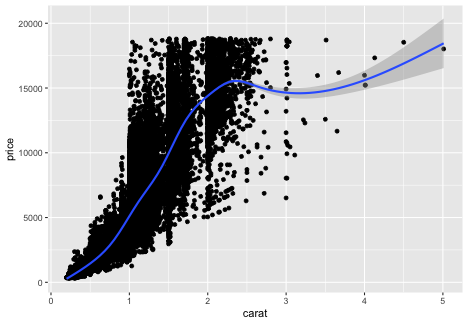
\includegraphics{_main_files/figure-latex/unnamed-chunk-14-1.png}

Die Layer-Funktionen können durch Parameter angepasst werden:

\begin{Shaded}
\begin{Highlighting}[]
\FunctionTok{ggplot}\NormalTok{(diamonds, }\FunctionTok{aes}\NormalTok{(}\AttributeTok{x =}\NormalTok{ carat, }\AttributeTok{y =}\NormalTok{ price)) }\SpecialCharTok{+}
  \FunctionTok{geom\_point}\NormalTok{(}\AttributeTok{size =} \FloatTok{0.5}\NormalTok{) }\SpecialCharTok{+}
  \FunctionTok{geom\_smooth}\NormalTok{(}\AttributeTok{color =} \StringTok{"red"}\NormalTok{)}
\end{Highlighting}
\end{Shaded}

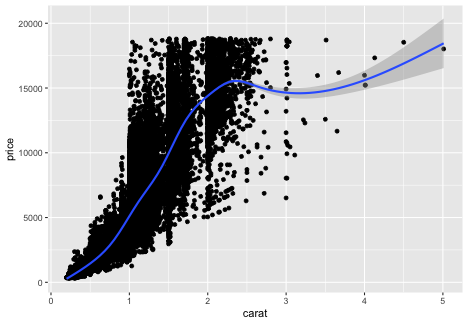
\includegraphics{_main_files/figure-latex/unnamed-chunk-15-1.png}

Dabei lassen sich in den einzelnen Layers mappings hinzufügen oder verändern:

\begin{Shaded}
\begin{Highlighting}[]
\FunctionTok{ggplot}\NormalTok{(diamonds, }\FunctionTok{aes}\NormalTok{(}\AttributeTok{x =}\NormalTok{ carat, }\AttributeTok{y =}\NormalTok{ price)) }\SpecialCharTok{+}
  \FunctionTok{geom\_point}\NormalTok{(}\FunctionTok{aes}\NormalTok{(}\AttributeTok{color =}\NormalTok{ clarity), }\AttributeTok{size =} \FloatTok{0.5}\NormalTok{) }\SpecialCharTok{+}
  \FunctionTok{geom\_smooth}\NormalTok{(}\AttributeTok{color =} \StringTok{"red"}\NormalTok{)}
\end{Highlighting}
\end{Shaded}

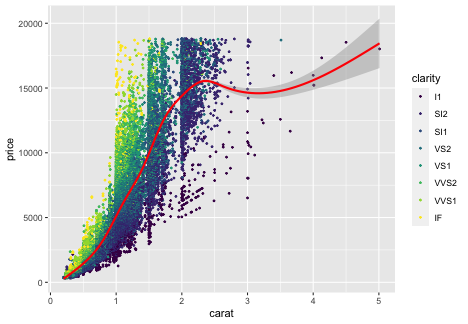
\includegraphics{_main_files/figure-latex/unnamed-chunk-16-1.png}

Schließlich lassen sich noch viele weitere optische Aspekte anpassen, z.B. Achsen, Farben, etc.:

\begin{Shaded}
\begin{Highlighting}[]
\FunctionTok{ggplot}\NormalTok{(diamonds, }\FunctionTok{aes}\NormalTok{(}\AttributeTok{x =}\NormalTok{ carat, }\AttributeTok{y =}\NormalTok{ price)) }\SpecialCharTok{+}
  \FunctionTok{geom\_point}\NormalTok{(}\FunctionTok{aes}\NormalTok{(}\AttributeTok{color =}\NormalTok{ clarity), }\AttributeTok{size =} \FloatTok{0.5}\NormalTok{) }\SpecialCharTok{+}
  \FunctionTok{geom\_smooth}\NormalTok{(}\AttributeTok{color =} \StringTok{"red"}\NormalTok{) }\SpecialCharTok{+}
  \FunctionTok{scale\_x\_continuous}\NormalTok{(}\StringTok{"Karatzahl"}\NormalTok{, }\AttributeTok{breaks =} \FunctionTok{seq}\NormalTok{(}\DecValTok{0}\NormalTok{, }\DecValTok{5}\NormalTok{, }\FloatTok{0.5}\NormalTok{)) }\SpecialCharTok{+}
  \FunctionTok{scale\_y\_continuous}\NormalTok{(}\StringTok{"Preis"}\NormalTok{) }\SpecialCharTok{+}
  \FunctionTok{scale\_color\_brewer}\NormalTok{(}\StringTok{"Klarheit"}\NormalTok{) }\SpecialCharTok{+}
  \FunctionTok{theme\_dark}\NormalTok{()}
\end{Highlighting}
\end{Shaded}

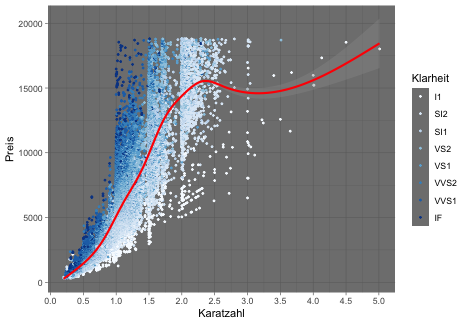
\includegraphics{_main_files/figure-latex/unnamed-chunk-17-1.png}

\hypertarget{aufgaben}{%
\subsection{Aufgaben}\label{aufgaben}}

\begin{enumerate}
\def\labelenumi{\arabic{enumi}.}
\item
  Versuchen Sie, die folgenden Visualisierungen des Datensatzes \texttt{diamonds} auszugeben:

  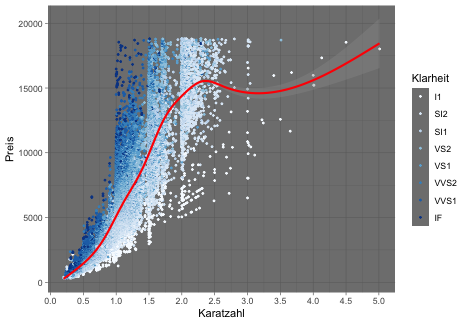
\includegraphics{_main_files/figure-latex/unnamed-chunk-18-1.png}

  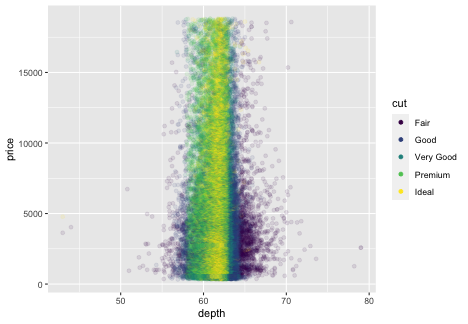
\includegraphics{_main_files/figure-latex/unnamed-chunk-19-1.png}

  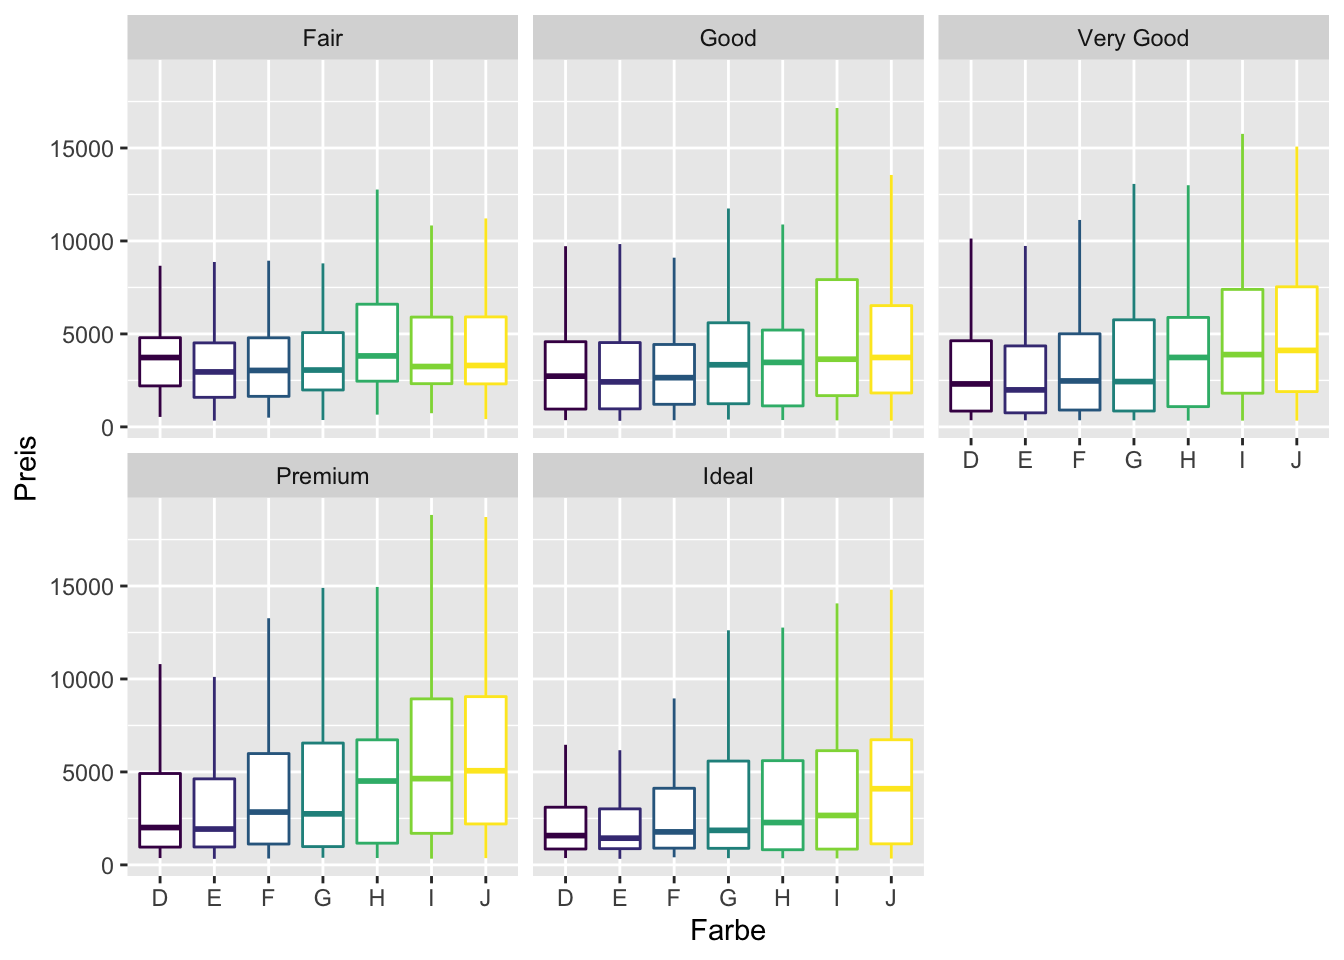
\includegraphics{_main_files/figure-latex/unnamed-chunk-20-1.png}
\item
  Schauen Sie sich die Publikation \href{https://r4ds.had.co.nz/}{R for Data Science} an.
\item
  Was ist das für ein Buch? Wer ist das Zielpublikum?
\item
  Lesen Sie das Kapitel ``3: Data Visualization'' und vollziehen Sie die Visualisierungen nach.
\item
  Bearbeiten Sie die Aufgaben.
\item
  Bearbeiten Sie die \href{https://rstudio.cloud/learn/primers/3}{RStudio Primers zu Datenvisualisierung}.
\end{enumerate}

\hypertarget{karten-erstellen-ftr}{%
\section{Karten erstellen (FTR)}\label{karten-erstellen-ftr}}

\hypertarget{lernziele-dieser-sitzung-1}{%
\subsection{Lernziele dieser Sitzung}\label{lernziele-dieser-sitzung-1}}

Sie können\ldots{}

\begin{itemize}
\tightlist
\item
  Pipes benutzen
\item
  einfache \texttt{dplyr}-Befehle ausführen
\item
  Koordinaten visualisieren
\end{itemize}

\hypertarget{voraussetzungen-1}{%
\subsection{Voraussetzungen}\label{voraussetzungen-1}}

Wir laden erstmal \texttt{tidyverse}:

\begin{Shaded}
\begin{Highlighting}[]
\FunctionTok{library}\NormalTok{(tidyverse)}
\end{Highlighting}
\end{Shaded}

\hypertarget{exkurs-pipes}{%
\subsection{Exkurs: Pipes}\label{exkurs-pipes}}

Teil vom \texttt{tidyverse} ist auch das Paket \texttt{magrittr}, das einen besonderen Operator enthält: \texttt{\%\textgreater{}\%}

Der Operator \texttt{\%\textgreater{}\%} heißt ``Pipe'' und setzt das Ergebnis der vorherigen Funktion als ersten Parameter in die nächste Funktion ein. Zur Veranschaulichung:

\begin{Shaded}
\begin{Highlighting}[]
\NormalTok{anzahl\_buchstaben }\OtherTok{\textless{}{-}} \FunctionTok{length}\NormalTok{(letters)}
\FunctionTok{sqrt}\NormalTok{(anzahl\_buchstaben)}
\end{Highlighting}
\end{Shaded}

\ldots ist das gleiche wie\ldots{}

\begin{Shaded}
\begin{Highlighting}[]
\FunctionTok{sqrt}\NormalTok{(}\FunctionTok{length}\NormalTok{(letters))}
\end{Highlighting}
\end{Shaded}

\ldots ist das gleiche wie\ldots{}

\begin{Shaded}
\begin{Highlighting}[]
\FunctionTok{length}\NormalTok{(letters) }\SpecialCharTok{\%\textgreater{}\%}
  \FunctionTok{sqrt}\NormalTok{()}
\end{Highlighting}
\end{Shaded}

\ldots ist das gleiche wie\ldots{}

\begin{Shaded}
\begin{Highlighting}[]
\NormalTok{letters }\SpecialCharTok{\%\textgreater{}\%}
\NormalTok{  length }\SpecialCharTok{\%\textgreater{}\%}
  \FunctionTok{sqrt}\NormalTok{()}
\end{Highlighting}
\end{Shaded}

So können beliebig viele Funktionen aneinandergereiht werden. Und mit \texttt{-\textgreater{}} kann eine Variable „in die andere Richtung`` zugewiesen werden

\begin{Shaded}
\begin{Highlighting}[]
\NormalTok{letters }\SpecialCharTok{\%\textgreater{}\%}
  \FunctionTok{length}\NormalTok{() }\SpecialCharTok{\%\textgreater{}\%}
  \FunctionTok{sqrt}\NormalTok{() }\SpecialCharTok{\%\textgreater{}\%}
  \FunctionTok{round}\NormalTok{() }\SpecialCharTok{\%\textgreater{}\%}
  \FunctionTok{as.character}\NormalTok{() }\OtherTok{{-}\textgreater{}}
\NormalTok{  my\_var}
\end{Highlighting}
\end{Shaded}

Gerade bei komplizierteren Zusammenhängen wird der Code so oft lesbarer, weil die Logik von links nach rechts, bzw. von oben nach unten gelesen werden kann.

\hypertarget{daten-importieren}{%
\subsection{Daten importieren}\label{daten-importieren}}

Beim Open-Data-Portal der Stadt Frankfurt steht ein \href{http://offenedaten.frankfurt.de/dataset/baumkataster-frankfurt-am-main}{Baumkataster} zur Verfügung.

Die Datei im CSV-Format (comma separated values) kann entweder heruntergeladen und durch klicken importiert werden, oder direkt über den Befehl:

\begin{Shaded}
\begin{Highlighting}[]
\NormalTok{baumkataster }\OtherTok{\textless{}{-}} \FunctionTok{read\_csv2}\NormalTok{(}\StringTok{"http://offenedaten.frankfurt.de/dataset/73c5a6b3{-}c033{-}4dad{-}bb7d{-}8783427dd233/resource/7a73520b{-}961a{-}4aad{-}a582{-}449e676c247c/download/gprojekteopen{-}datadatenamt{-}67datenbaumauswahl\_veroffentlichung\_4baumauswahl\_veroffentlichung\_4.csv"}\NormalTok{)}
\end{Highlighting}
\end{Shaded}

\hypertarget{uxfcberblick-verschaffen}{%
\subsection{Überblick verschaffen}\label{uxfcberblick-verschaffen}}

Mit \texttt{summary()} lässt sich eine Zusammenfassung der Werte generieren:

\begin{Shaded}
\begin{Highlighting}[]
\FunctionTok{summary}\NormalTok{(baumkataster)}
\DocumentationTok{\#\#  Gattung/Art/Deutscher Name   Baumnummer         Objekt            Pflanzjahr  }
\DocumentationTok{\#\#  Length:118403              Min.   :    1.0   Length:118403      Min.   :1645  }
\DocumentationTok{\#\#  Class :character           1st Qu.:   24.0   Class :character   1st Qu.:1970  }
\DocumentationTok{\#\#  Mode  :character           Median :   82.0   Mode  :character   Median :1982  }
\DocumentationTok{\#\#                             Mean   :  232.7                      Mean   :1979  }
\DocumentationTok{\#\#                             3rd Qu.:  270.0                      3rd Qu.:1995  }
\DocumentationTok{\#\#                             Max.   :20158.0                      Max.   :2017  }
\DocumentationTok{\#\#                             NA\textquotesingle{}s   :1853                                       }
\DocumentationTok{\#\#  Kronendurchmesser    HOCHWERT         RECHTSWERT    }
\DocumentationTok{\#\#  Min.   : 2.000    Min.   :5545117   Min.   :463163  }
\DocumentationTok{\#\#  1st Qu.: 4.000    1st Qu.:5550428   1st Qu.:472715  }
\DocumentationTok{\#\#  Median : 6.000    Median :5552601   Median :475219  }
\DocumentationTok{\#\#  Mean   : 6.688    Mean   :5552953   Mean   :475244  }
\DocumentationTok{\#\#  3rd Qu.: 9.000    3rd Qu.:5555165   3rd Qu.:478201  }
\DocumentationTok{\#\#  Max.   :63.000    Max.   :5563639   Max.   :485361  }
\DocumentationTok{\#\# }
\end{Highlighting}
\end{Shaded}

Genauere Infos über diese Merkmale gibt es auf dem Datenportal.

\hypertarget{visualisieren}{%
\subsection{Visualisieren}\label{visualisieren}}

Wie in der letzten Lektion besprochen, lässt sich der Datensatz mit \texttt{ggplot()} visualisieren, z.~B.:

\begin{Shaded}
\begin{Highlighting}[]
\FunctionTok{ggplot}\NormalTok{(baumkataster, }\FunctionTok{aes}\NormalTok{(}\AttributeTok{x =}\NormalTok{ Kronendurchmesser)) }\SpecialCharTok{+}
  \FunctionTok{geom\_histogram}\NormalTok{()}
\end{Highlighting}
\end{Shaded}

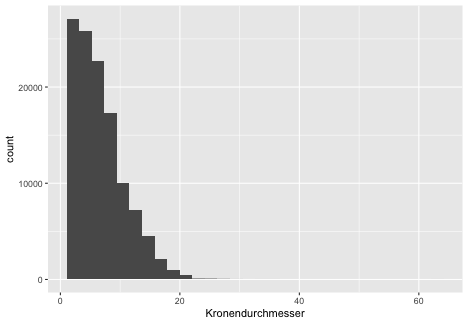
\includegraphics{_main_files/figure-latex/unnamed-chunk-29-1.png}

Eine neue Messreihe lässt sich z.~B. so errechnen:

\begin{Shaded}
\begin{Highlighting}[]
\NormalTok{alter }\OtherTok{\textless{}{-}} \DecValTok{2020} \SpecialCharTok{{-}}\NormalTok{ baumkataster}\SpecialCharTok{$}\NormalTok{Pflanzjahr}
\FunctionTok{head}\NormalTok{(alter)}
\DocumentationTok{\#\# [1] 100 100 100 100 100 100}
\end{Highlighting}
\end{Shaded}

Der Befehl \texttt{mutate()} funktioniert sehr ähnlich, gibt aber den veränderten Datensatz zurück:

\begin{Shaded}
\begin{Highlighting}[]
\FunctionTok{mutate}\NormalTok{(baumkataster, }\AttributeTok{alter =} \DecValTok{2020} \SpecialCharTok{{-}}\NormalTok{ Pflanzjahr)}
\DocumentationTok{\#\# \# A tibble: 118,403 x 8}
\DocumentationTok{\#\#    \textasciigrave{}Gattung/Art/Deutsch\textasciitilde{} Baumnummer Objekt  Pflanzjahr Kronendurchmess\textasciitilde{} HOCHWERT}
\DocumentationTok{\#\#    \textless{}chr\textgreater{}                      \textless{}dbl\textgreater{} \textless{}chr\textgreater{}        \textless{}dbl\textgreater{}            \textless{}dbl\textgreater{}    \textless{}dbl\textgreater{}}
\DocumentationTok{\#\#  1 Platanus x hispanica\textasciitilde{}          1 Ackerm\textasciitilde{}       1920                8 5549511.}
\DocumentationTok{\#\#  2 Platanus x hispanica\textasciitilde{}          2 Ackerm\textasciitilde{}       1920                8 5549517.}
\DocumentationTok{\#\#  3 Platanus x hispanica\textasciitilde{}          3 Ackerm\textasciitilde{}       1920                8 5549524.}
\DocumentationTok{\#\#  4 Platanus x hispanica\textasciitilde{}          4 Ackerm\textasciitilde{}       1920                8 5549531 }
\DocumentationTok{\#\#  5 Platanus x hispanica\textasciitilde{}          5 Ackerm\textasciitilde{}       1920                8 5549538.}
\DocumentationTok{\#\#  6 Platanus x hispanica\textasciitilde{}          6 Ackerm\textasciitilde{}       1920                8 5549544.}
\DocumentationTok{\#\#  7 Platanus x hispanica\textasciitilde{}          7 Ackerm\textasciitilde{}       1920                8 5549551.}
\DocumentationTok{\#\#  8 Platanus x hispanica\textasciitilde{}          8 Ackerm\textasciitilde{}       1920                8 5549557.}
\DocumentationTok{\#\#  9 Platanus x hispanica\textasciitilde{}          9 Ackerm\textasciitilde{}       1920                8 5549564.}
\DocumentationTok{\#\# 10 Platanus x hispanica\textasciitilde{}         10 Ackerm\textasciitilde{}       1920                8 5549571.}
\DocumentationTok{\#\# \# ... with 118,393 more rows, and 2 more variables: RECHTSWERT \textless{}dbl\textgreater{},}
\DocumentationTok{\#\# \#   alter \textless{}dbl\textgreater{}}
\end{Highlighting}
\end{Shaded}

Derselbe Befehl mit dem Pipe-Operator:

\begin{Shaded}
\begin{Highlighting}[]
\NormalTok{baumkataster }\SpecialCharTok{\%\textgreater{}\%}
  \FunctionTok{mutate}\NormalTok{(}\AttributeTok{alter =} \DecValTok{2020} \SpecialCharTok{{-}}\NormalTok{ Pflanzjahr)}
\DocumentationTok{\#\# \# A tibble: 118,403 x 8}
\DocumentationTok{\#\#    \textasciigrave{}Gattung/Art/Deutsch\textasciitilde{} Baumnummer Objekt  Pflanzjahr Kronendurchmess\textasciitilde{} HOCHWERT}
\DocumentationTok{\#\#    \textless{}chr\textgreater{}                      \textless{}dbl\textgreater{} \textless{}chr\textgreater{}        \textless{}dbl\textgreater{}            \textless{}dbl\textgreater{}    \textless{}dbl\textgreater{}}
\DocumentationTok{\#\#  1 Platanus x hispanica\textasciitilde{}          1 Ackerm\textasciitilde{}       1920                8 5549511.}
\DocumentationTok{\#\#  2 Platanus x hispanica\textasciitilde{}          2 Ackerm\textasciitilde{}       1920                8 5549517.}
\DocumentationTok{\#\#  3 Platanus x hispanica\textasciitilde{}          3 Ackerm\textasciitilde{}       1920                8 5549524.}
\DocumentationTok{\#\#  4 Platanus x hispanica\textasciitilde{}          4 Ackerm\textasciitilde{}       1920                8 5549531 }
\DocumentationTok{\#\#  5 Platanus x hispanica\textasciitilde{}          5 Ackerm\textasciitilde{}       1920                8 5549538.}
\DocumentationTok{\#\#  6 Platanus x hispanica\textasciitilde{}          6 Ackerm\textasciitilde{}       1920                8 5549544.}
\DocumentationTok{\#\#  7 Platanus x hispanica\textasciitilde{}          7 Ackerm\textasciitilde{}       1920                8 5549551.}
\DocumentationTok{\#\#  8 Platanus x hispanica\textasciitilde{}          8 Ackerm\textasciitilde{}       1920                8 5549557.}
\DocumentationTok{\#\#  9 Platanus x hispanica\textasciitilde{}          9 Ackerm\textasciitilde{}       1920                8 5549564.}
\DocumentationTok{\#\# 10 Platanus x hispanica\textasciitilde{}         10 Ackerm\textasciitilde{}       1920                8 5549571.}
\DocumentationTok{\#\# \# ... with 118,393 more rows, and 2 more variables: RECHTSWERT \textless{}dbl\textgreater{},}
\DocumentationTok{\#\# \#   alter \textless{}dbl\textgreater{}}
\end{Highlighting}
\end{Shaded}

So lassen sich auch hier verschiedene Befehle verknüpfen. \texttt{filter()} beschränkt den Datensatz auf Merkmalsträger, die den Kriterien entsprechen:

\begin{Shaded}
\begin{Highlighting}[]
\NormalTok{baumkataster }\SpecialCharTok{\%\textgreater{}\%}
  \FunctionTok{mutate}\NormalTok{(}\AttributeTok{alter =} \DecValTok{2020} \SpecialCharTok{{-}}\NormalTok{ Pflanzjahr) }\SpecialCharTok{\%\textgreater{}\%}
  \FunctionTok{filter}\NormalTok{(alter }\SpecialCharTok{\textgreater{}} \DecValTok{30}\NormalTok{) }\OtherTok{{-}\textgreater{}}
\NormalTok{  alte\_baeume}

\FunctionTok{summary}\NormalTok{(alte\_baeume)}
\DocumentationTok{\#\#  Gattung/Art/Deutscher Name   Baumnummer         Objekt            Pflanzjahr  }
\DocumentationTok{\#\#  Length:73859               Min.   :    1.0   Length:73859       Min.   :1645  }
\DocumentationTok{\#\#  Class :character           1st Qu.:   29.0   Class :character   1st Qu.:1960  }
\DocumentationTok{\#\#  Mode  :character           Median :   97.0   Mode  :character   Median :1974  }
\DocumentationTok{\#\#                             Mean   :  263.2                      Mean   :1966  }
\DocumentationTok{\#\#                             3rd Qu.:  314.0                      3rd Qu.:1980  }
\DocumentationTok{\#\#                             Max.   :10489.0                      Max.   :1989  }
\DocumentationTok{\#\#                             NA\textquotesingle{}s   :684                                        }
\DocumentationTok{\#\#  Kronendurchmesser    HOCHWERT         RECHTSWERT         alter       }
\DocumentationTok{\#\#  Min.   : 2.000    Min.   :5545117   Min.   :463163   Min.   : 31.00  }
\DocumentationTok{\#\#  1st Qu.: 6.000    1st Qu.:5550415   1st Qu.:472667   1st Qu.: 40.00  }
\DocumentationTok{\#\#  Median : 8.000    Median :5552480   Median :475708   Median : 46.00  }
\DocumentationTok{\#\#  Mean   : 8.503    Mean   :5552593   Mean   :475402   Mean   : 53.54  }
\DocumentationTok{\#\#  3rd Qu.:10.000    3rd Qu.:5554589   3rd Qu.:478539   3rd Qu.: 60.00  }
\DocumentationTok{\#\#  Max.   :35.000    Max.   :5563639   Max.   :485360   Max.   :375.00  }
\DocumentationTok{\#\# }
\end{Highlighting}
\end{Shaded}

Schließlich ergibt das Streudiagramm von Koordinaten so eine art Karte:

\begin{Shaded}
\begin{Highlighting}[]
\FunctionTok{ggplot}\NormalTok{(alte\_baeume) }\SpecialCharTok{+}
    \FunctionTok{geom\_point}\NormalTok{(}\AttributeTok{size =} \FloatTok{0.1}\NormalTok{, }\FunctionTok{aes}\NormalTok{(}\AttributeTok{x =}\NormalTok{ RECHTSWERT, }\AttributeTok{y =}\NormalTok{ HOCHWERT))}
\end{Highlighting}
\end{Shaded}

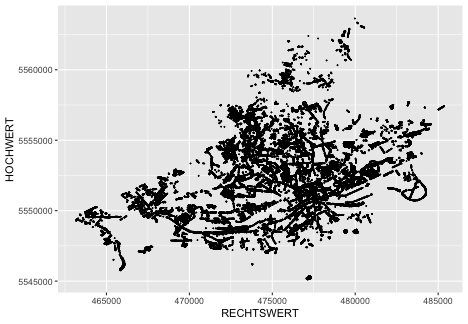
\includegraphics{_main_files/figure-latex/unnamed-chunk-34-1.png}

Diesen Ansatz werden wir in der nächsten Lektion vertiefen.

\hypertarget{karten-erstellen-hos}{%
\section{Karten erstellen (HOS)}\label{karten-erstellen-hos}}

\hypertarget{aufgaben-1}{%
\subsection{Aufgaben}\label{aufgaben-1}}

\begin{enumerate}
\def\labelenumi{\arabic{enumi}.}
\item
  Besuchen Sie \url{https://pleiades.stoa.org/} - worum geht es hier?
\item
  Finden Sie den kompletten aktuellen Datensatz für „locations`` als CSV-Datei.
\item
  Importieren Sie ihn in R und weisen Sie dem Datensatz den Namen \texttt{pleiades} zu.
\item
  Finden Sie geeignete Werte für (einzelne) Längen- und Breitengrade im Datensatz.
\item
  Plotten Sie die Koordinaten auf x- und y-Achse mit \texttt{ggplot()}. Was erkennen Sie?
\item
  Halbieren Sie die Größe und setzen Sie den Alpha-Wert der Punkte auf 0,2.
\item
  Bringen Sie die Grafik in die Mercator-Projektion.
\item
  Schauen Sie sich diesen Befehl an:

\begin{Shaded}
\begin{Highlighting}[]
\FunctionTok{map\_data}\NormalTok{(}\StringTok{"world"}\NormalTok{) }\SpecialCharTok{\%\textgreater{}\%}
  \FunctionTok{ggplot}\NormalTok{() }\SpecialCharTok{+}
    \FunctionTok{geom\_polygon}\NormalTok{(}\AttributeTok{mapping =} \FunctionTok{aes}\NormalTok{(}\AttributeTok{x =}\NormalTok{ long,}
                               \AttributeTok{y =}\NormalTok{ lat,}
                               \AttributeTok{group =}\NormalTok{ group)) }\SpecialCharTok{+}
    \FunctionTok{coord\_quickmap}\NormalTok{(}\AttributeTok{xlim =} \FunctionTok{c}\NormalTok{(}\SpecialCharTok{{-}}\DecValTok{8}\NormalTok{, }\DecValTok{40}\NormalTok{),}
                   \AttributeTok{ylim =} \FunctionTok{c}\NormalTok{(}\DecValTok{26}\NormalTok{, }\DecValTok{48}\NormalTok{))}
\end{Highlighting}
\end{Shaded}
\item
  Versuchen Sie, jede einzelne Zeile nachzuvollziehen, indem Sie die entsprechenden Funktionen recherchieren.
\item
  Führen Sie den Befehl aus.
\item
  Ändern Sie die Farbe der Flächen in hellgrau.
\item
  Wählen Sie einen Kartenausschnitt, auf dem Portugal, Ägypten, Irak und Frankreich komplett zu sehen sind.
\item
  Plotten Sie auf diesem Hintergrund den Datensatz \texttt{pleiades}. Passen Sie dabei die Parameter so an, dass es Ihnen optisch zusagt.
\item
  Wählen Sie für die Karte die \href{https://de.wikipedia.org/wiki/Bonnesche_Projektion}{Bonnesche Projektion} mit Standardparallele bei 40°N.
\item
  Entfernen Sie alle Achsenbeschriftungen.
\item
  (Achtung: knifflig!) Bilden Sie diese Grafik nach, die die Orte geordnet nach ältestem Fund darstellt:

  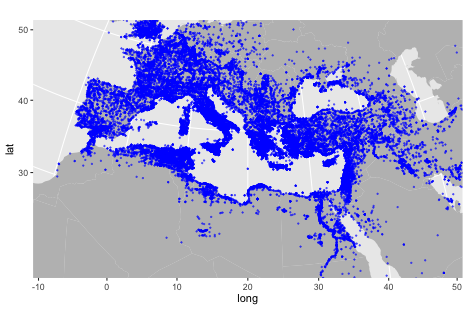
\includegraphics{_main_files/figure-latex/unnamed-chunk-47-1.png}
\end{enumerate}

\end{document}
